\section{Prototype}
\label{sec:mx}

%% \begin{figure}[t!]
%% \centering
%% \includegraphics[width=\columnwidth]{safe-updates/figures/overview}
%% \caption{A platform running both conventional and multi-version
%%   applications.}
%% \label{fig:mx-platform}
%% \end{figure}

We have implemented our approach in a prototype system called \mx,
targeted at multi-core processors running Linux.  Currently, \mx
supports two versions run in parallel. The system works directly on
application binaries, making it easy to deploy it and possibly integrate
it with existing software package managers such as \textstt{apt} or
\textstt{yum}.

%Figure~\ref{fig:mx-platform} shows a platform running \mx, on which
On a platform using \mx, conventional (\ie unmodified) applications
and multi-version (\mv) applications run side by side.  The key
property that must hold on such a platform is that without purposely
trying to do so, applications should not be able to distinguish
between conventional and \mv applications running on the platform. In
particular, the multiple versions of an \mv application should appear
as one to any other entity interacting with them (\eg user, operating
system, other machines).  Furthermore, \mv applications should be more
reliable and secure than their component versions, and their
performance should not be significantly degraded.

To achieve these goals, our prototype \mx employs several different
components, as shown in the architectural overview of
Figure~\ref{fig:design}.  The input to \mx consists of the binaries of
two versions of an application, which we will refer to as 
\textit{the old version}---the one already running on the system, and 
\textit{the new version}---the one newly released.


These two binaries are first statically analysed by the \sea (Static
Executable Analyser) component, which constructs a mapping from the
control flow graph (CFG) of the old version to the CFG of the new
version (\S\ref{sec:sea}).  The two versions are then passed to \mxm
(Multi-eXecution Monitor), whose job is to run the two versions in
parallel, synchronise their execution, virtualise their interaction
with the outside environment, and detect any divergences in their
external behaviour (\S\ref{sec:mxm}).  Once a divergence is detected,
it is resolved by \rem (Runtime Execution Manipulator), which selects
between the available behaviours, and resynchronises the two versions
after the divergence (\S\ref{sec:rem}).

The system prototype has been implemented in C with a small amount of
assembly, and the current version has approximately \mxSLOC source
lines of code. The implementation currently supports Linux kernels
3.2.0 and above, running x86 and x86-64 architectures.

The rest of this section describes the main \mx system components and
their implementation in more detail, and discusses how they work
together to support safe software updates.

\begin{figure}[t!]
\begin{center}
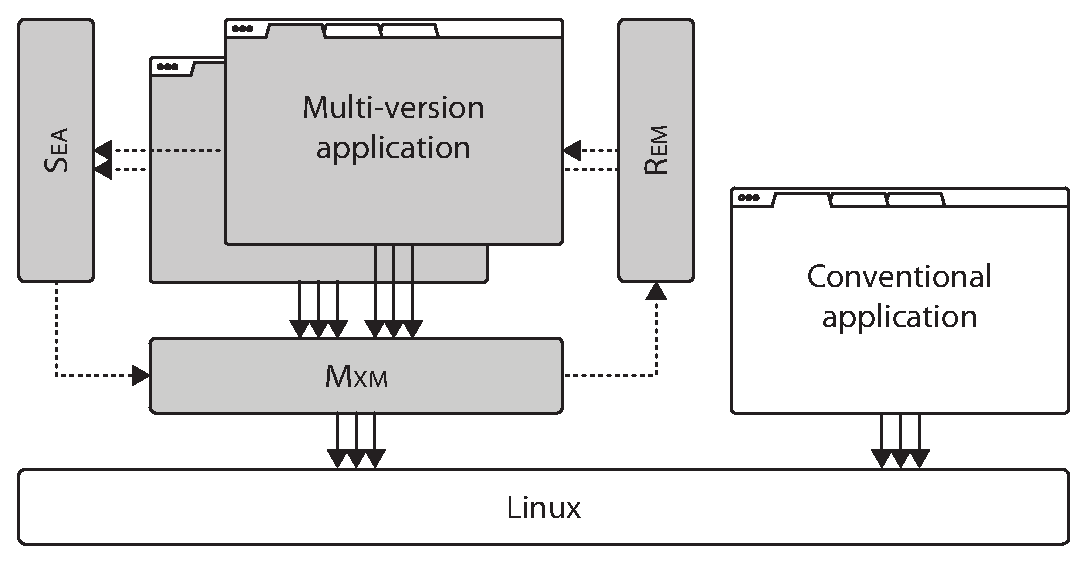
\includegraphics[width=0.5\columnwidth]{safe-updates/figures/architecture}
\caption{\mx system architecture.  
%% The main components of \mx
%%   are \sea (Static Executable Analyser), \mxm (Multi-eXecution
%%   Monitor), and \rem (Runtime Execution Manipulator).
}
\label{fig:design}
\end{center}
\end{figure}


\subsection{System call interposition}
\label{sec:mxm}

One of the main components of our multi-version execution environment
is the \mxm monitor.  \mxm's main jobs are to run the two versions
concurrently, mediate their interaction with the outside world,
synchronise their executions, and detect any divergences in their
external behaviour. \mxm works by intercepting all system calls issued
by each application version, and manipulating them to ensure that the
two versions are executed in a synchronised fashion and act as one to
the outside world.

\mxm provides functionality similar to conventional virtual machine
monitors.  Whenever the MV application is executed, the \mxm connects
to all application versions running in parallel, intercepting their
kernel system calls.  \mxm ensures that the two versions act as one to
the outside world by mediating access to the underlying operating
system to achieve complete isolation of the running application from
other application instances as well as from the external environment,
making sure the combined application versions act as one to the
outside world.  The environment controlled by the monitor consists
mainly of a restricted file system access, socket interceptors and
signal handlers.

\subsubsection{System call interception}

\mxm is implemented using the  \ptrace interface provided by the Linux
kernel.  This interface, often used for application debugging, allows
simple deployment (without any need for compile-time instrumentation)
and makes the monitor itself lightweight since it is running as a
regular unprivileged process.  \mxm is similar in operation to previous
monitors whose goal is to synchronise applications at the level of system
calls such as Orchestra~\cite{orchestra09}, PLR~\cite{shye2009} or
Tachyon~\cite{tachyon12}.

\mxm runs each version in a separate child process, intercepting all
their system calls.  When a system call is intercepted in one version,
\mxm waits until the other version also performs a system call.  With
a pair of system calls in hand (one executed by the old version, and
one by the new version), \mxm compares their types and arguments.  If
they differ, \mxm has detected a divergence and invokes the \rem
component to resolve it (\S\ref{sec:rem}).

Otherwise, if the two versions perform the same system call with the
same arguments, \mxm virtualises their interaction with the
environment.  If the operation performed by the system call has no
side effects and does not involve virtualised state (\eg
\textstt{sysinfo}), \mxm allows both processes to execute it
independently.  Otherwise, it executes the system call on their
behalf and copies its results into the address spaces of both
versions.

\mxm must also enforce deterministic execution across versions. This
consists mainly of intercepting instructions that may produce
non-deterministic results, and returning the same result in both
versions.  Examples of such non-deterministic operations include
random number generators (\eg read calls to \textstt{/dev/[u]random}),
date and time (\eg read calls to \textstt{/etc/localtime}), and access
to files and network (\eg file descriptor consistency).  Note that
non-deterministic effects resulting from allocating memory objects at
different addresses in memory or randomly arranging memory areas via
address space layout randomisation (ASLR) do not pose any
problems: \mxm understand the semantics of individual system calls and
rather than directly comparing memory addresses (which might be
different in each executed version), it compares the actual values
stored at those memory locations. \mxm support both memory buffers (by
comparing the actual buffer content) as well as data structures
referenced by pointers (including nested ones).
 
Since \mxm fully controls executing programs intercepting all their
system calls, it can ensure that both programs have the same view of
their environment.

Whenever the monitored process makes a system call, \mxm is notified
twice---first before, then after the call has been executed.  When a
\ptrace event is raised (\eg a new child process has been started),
the monitor is notified as well.  Due to internal limitations of the
\ptrace interface, once the system call has been made, it cannot be
skipped, so when \mxm wants to execute the call on behalf of its child
processes, it simply replaces it with a system call that does not
change the system state (\texttt{getpid} in our case).

There are several challenges that we encountered while implementing
\mxm.  First, \mxm must partly understand the semantics of 
system calls.  For example, many system call parameters use complex
(often nested) structures with complicated semantics to pass values to
the operating system kernel, as in the case of \textstt{ioctl} or
\textstt{futex}.  To be able to compare the parameters of
these system calls and copy back their results, \mxm needs to
understand the semantics of these structures.  However, there are only
a relatively small number of system calls in Linux, and once the support
for handling them is implemented, it can be reused across applications.
\mxm currently implements \syscallsImplemented system calls (out of the
\syscallsTotal provided by Linux x86-64 3.1.9), which was enough to
allow us to run \mx on our benchmarks
(\S\ref{sec:evaluation}).

Second, the arguments of a system call are often passed through pointers,
which are only valid in the application address space, which is not directly
available to \mxm.  Therefore, \mxm needs to copy the contents pointed to by
these structures to its own address space in order to perform their
comparison.  The \ptrace interface on x86-64 only allows to copy one quadword
per system call, which is very expensive. Previous approaches either used
various ad-hoc optimisations~\cite{orchestra09} such as named pipes or shared
memory with custom shellcode, or a modified kernel~\cite{tachyon12} to
overcome this limitation. Instead, \mxm uses \emph{cross memory attach}, a new
mechanism for fast interprocess communication which has been recently added to
the Linux kernel~\cite{crossmemoryattach}.  This mechanism provides two new
system calls---\textstt{process\_vm\_readv} and
\textstt{process\_vm\_writev}---which allows tracer to directly access the
memory space of tracee using an interface similar to \textstt{readv} and
\textstt{writev} system calls without any additional overhead.

Third, because the structures passed as arguments to system calls often have
variable-size, \mxm also needs a fast way to allocate and deallocate memory
for them in order to minimise the overall overhead imposed by our system.  For
this purpose, \mxm uses a region-based memory allocator~\cite{memory-pools},
namely the \textstt{obstack}
library\footnote{\url{http://www.gnu.org/software/hello/manual/libc/Obstacks.html}}.
which is part of the GNU C Library.  Each monitored process has its own
obstack, which is used for allocating memory to store the copy of the process'
system call arguments

\subsubsection{Multi-process and multi-threaded applications}

Finally, a particular challenge arises in the context of multi-process and
multi-threaded applications.  Using a single monitor instance to intercept both
versions and their child processes (or threads) would eliminate any advantage
that these applications derive from using concurrency.  Therefore, \mxm uses a
new monitor thread for each set of child processes (or threads) spawned by the
application.  For instance, if the old and new versions each have a parent and
a child process, then \mxm will use two threads: one to monitor the parent
processes, and one to monitor the child processes in each version.

Due to limitations of the \ptrace interface (which was not designed to be used
in a multi-process/multi-threaded environment), handing the control of any
child processes being spawned by the application over to a new monitoring
thread is somewhat complicated.  In \mxm we adopt the solution similar to
Orchestra~\cite{orchestra09}.  When a new child process is spawned, we let the
parent monitoring thread to supervise its execution until the first system
call.  Then, we replace this system call with a \textstt{pause} system call,
disconnect the parent monitor (which causes a \textstt{continue} signal to be
sent to all new child processes), and spawn a new monitoring thread which
immediately reconnects to the new child process, restores its original system
call, and resumes its execution.

\mxm does not enforce deterministic execution across multiple versions of
multi-threaded programs (which may diverge if race conditions can lead
to different external behaviour across executions), although we could
overcome this limitation by adopting \varan's solution
(\S\ref{sec:threading}).

%% \mxm also performs a series of optimisations to decrease performance
%% overhead, such as allowing certain files with read-only permissions
%% to be opened directly by the process. 

\subsubsection{Environment virtualisation}

To improve I/O performance and decrease virtualisation overhead,
processes are allowed to open files with read-only permissions
directly, while files with write permissions are opened by the monitor
itself.  This imposes another problem as file descriptors assigned to
these files are not necessarily the same in each version (\eg due to
scheduling non-determinism). Therefore, the \mxm needs to virtualise
these file descriptors.

Whenever monitored process opens a file with read-only permissions, a
new virtual file descriptor is assigned to this file together with the
mapping to a real file descriptor for each version. This virtual file
descriptor is then send to each version. When system call is made
using this virtual file descriptor, \mxm replaces it with the real
file descriptor before executing the system call. The actual file
operation is then executed by the process itself avoiding any memory
copying by \mxm.

A similar approach is also used for virtualisation of process,
group, parent and child identifiers.  Whenever a process tries to obtain
the actual ID, \mxm replaces this with a virtual ID and keeps the
mapping between the real and the virtual ID. When a process invokes a
system call using this ID as an argument (\eg \texttt{kill}), the
virtual ID is replaced with the actual ID before executing the system
call.

%% \paragraph{Para-virtualisation interface and binary translation.}
%% Furthermore, we plan to combine this API with a binary translation
%% approach~\cite{binary-translation}, that will allow to dynamically
%% replace certain system calls with more efficient \emph{monitor
%% call} instructions.  The binary translation could be also used to
%% dynamically replace code components that have been proved to be
%% safe and do not need to be replicated across multiple versions (\eg
%% using static verification during compilation, using traces of
%% previous execution, using runtime heuristics).


%% \paragraph{Future work}

%% The \texttt{ptrace} interface allows us to easily monitor the program
%% execution without any compile-time instrumentation.  The main downside
%% of this approach is a relatively high overhead.  This is especially
%% true for I/O intensive applications, as they require frequent
%% transfers of large portions of the application memory space to the
%% monitor process. This overhead could be eliminated by directly
%% accessing the process memory space.

%% The existing prototype implementation of \textsc{Mxm} already supports
%% simple scenarios. The main limitation of this implementation is the
%% strict ordering of system calls, which must be the same in each
%% monitored application version.  To be practically usable, future
%% versions of \textsc{Mxm} need to relax the requirement on strict
%% ordering to allow more complex scenarios. This is especially important
%% when executing different versions of the same application.

%% Most importantly, a straightforward comparison of system call traces
%% is usually not sufficient to identify divergences, since different
%% versions might use a slightly different sequence of kernel and library
%% calls to implement the same behaviour.  We plan to explore approaches
%% similar to those implemented by compiler optimisations, such as
%% \emph{peep-hole optimisation}~\cite{dragon-book}, and adapt them to
%% work on the level of kernel and library calls.


%% %% \paragraph{Hashing system call traces.}
%% %% To decrease the overhead of kernel and library call synchronisation, we aim to
%% %% enhance our system to hash the sequence of system call traces using fast hash
%% %% functions such as FNV-1 or FNV-1a.  This approach has a significant advantage
%% %% over straightforward comparison of call traces, especially in the case of
%% %% system calls with virtually unlimited parameter sizes such as \texttt{read} or
%% %% \texttt{write}~\cite{shye2009}.  Similar approach has been already used
%% %% in~\cite{shye2009}.

%% \paragraph{Libraries support and virtualisation.}
%% Since many applications today use functionality provided by shared
%% libraries, we aim to support intercepting calls to such libraries as
%% well. Moreover, as intercepted calls to shared libraries can be
%% executed only once, same as in the case of system call monitoring,
%% this may decrease the overall overhead of multi-version execution.

%% We also plan to provide our own implementation of the \texttt{libc}
%% library loaded using the \texttt{LD\_PRELOAD} mechanism.  This library
%% will communicate directly with the monitor process through shared
%% memory, decreasing the number of system calls that need to be directly
%% intercepted, and thus resulting in much better performance.  However,
%% since the \texttt{LD\_PRELOAD} mechanism can be overridden, we still
%% need to combine it with the \texttt{ptrace} monitoring facility to
%% achieve complete isolation with reasonable overhead.  This approach
%% can be extended to support other shared libraries as well, further
%% improving the overall performance of our approach.

\subsection{Runtime state manipulation}
\label{sec:rem}

At the core of our system lies the \rem component, which is invoked
by \mxm whenever a divergence is detected.  \rem has two main jobs:
(1)~to decide whether to resolve the divergence in favour of the old or
the new version; and (2)~to allow the other version to execute through
the divergence and resynchronise the execution of the two versions
after the divergence.
%% The first task by itself it's easy: we favour the new version, except
%% for when it crashes.
%% As discussed in \sref{sec:scope}, in this paper we restrict our
%% attention to surviving crash errors, so the first task is relatively
%% easy: if one of the two versions crashes, we use the output of the
%% other version; otherwise, we always favour the new version.  
%%
%% The second task is however more difficult, but essential to the
%% success of our approach, which relies on having both versions be alive
%% at all times, so that the overall application can survive any crash
%% bugs that happen in either the old or the new version (although of
%% course, not in both).
%%
As discussed in Section~\ref{multi-version:rationale}, in \mx we focus
our attention on surviving crash errors, so the key challenge is to
allow the crashing version to survive the crash.  This is essential to
the success of our approach, which relies on having both versions alive
at all times, so that the overall application can survive any crash bugs
that happen in either the old or the new version (although of course,
not in both at the same time).

We emphasise that we apply our approach only to crash errors (those
raising a \textstt{SIGSEGV} signal), and not to other types of program
termination, such as \textstt{abort}s.  This is important from a
security perspective, because
%% many patches turn potential compromises into
%% run-time {\small{\texttt{abort}s}}, \eg using assertions for input
%% sanitisation.  For example, 
when a vulnerability is discovered, but a proper solution is not yet
known, developers often
\footnote{For example, see the patch in json-cpp \url{http://jsoncpp.svn.sourceforge.net/viewvc/jsoncpp/trunk/jsoncpp/include/json/assertions.h?r1=247&r2=246&pathrev=247}}
fail-stop the program rather than letting it continue and allowing
the attacker to compromise the system.\looseness=-1
%
%% Such situations can be easily distinguished since failed assertions
%% result in program abortion (\ie
%% \textstt{SIGABRT} signal), while unintentional program crashes typically
%% result in abnormal termination (\ie \textstt{SIGSEGV} signal). 
%% Therefore, \rem only intercepts and handles crashes resulting
%%   in \textstt{SIGSEGV} signals.

Suppose that one of the versions has crashed between the execution of
system call $s_1$ and the execution of system call $s_2$.  Then, in
many common scenarios, the code executed between the two system calls
is responsible for the crash (\eg the old version crashes because it
doesn't incorporate a bug fix present in the new version, or the new
version crashes because its code was patched incorrectly).  Therefore,
our strategy is to do a form of \textit{runtime code patching}, in
which we use the code of the non-crashing version to execute over the
buggy code in the crashing version.

%% If the behaviour of the two versions is different, but they both
%% continue to execute, then we favour the behaviour of the new version and
%% wait for the two versions to reconverge.

%% There are many different ways to achieve this goal, such as the use of
%% a mechanism based on check-pointing and roll-back~\cite{qin2005};
%% however, these mechanisms cannot deal with persistent errors which are
%% common in the case of software updates.

%% Our solution is based upon the observation that errors in programs are
%% usually located at particular places (\ie specific instructions) in
%% the program's code.  Therefore, we can use the code of the other, and
%% \ie correct, version to execute over this critical point in program's
%% code. This approach may not work when memory layout of the two
%% versions differs, as the code of one version may fail to locate the
%% memory structures necessary for its execution in the memory of the
%% other version. Nevertheless, the described approach might still work
%% in many cases when memory layout of the two versions does not differ
%% significantly.


%\paragraph{Possible execution scenarios.}

%% We run two versions of the same application in parallel, monitoring
%% their execution to be sure that they behave in the same way without
%% any divergences by comparing the application executions at
%% synchronisation points; in case of our prototype equal to system
%% calls. When either of the versions fail, we stop its execution at the
%% \emph{divergence point}; at this point there are three possible
%% solutions to synchronise the divergent versions:

\begin{figure}[t]
\centering
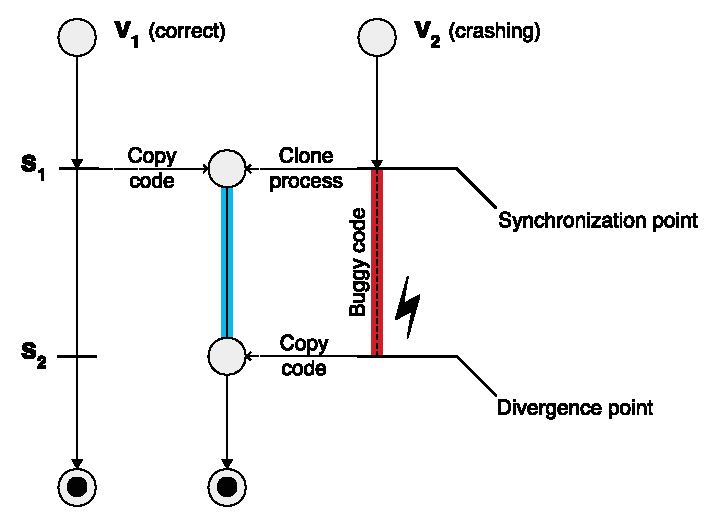
\includegraphics[width=0.5\columnwidth]{safe-updates/figures/strategy}
\caption{\rem's recovery mechanism uses the code of the non-crashing
  version to run through the buggy code.}
\label{fig:solution3}
\end{figure}

%% \begin{enumerate}[label=\emph{S\arabic*}, itemsep=3pt, parsep=3pt]
%% \renewcommand*\labelitemi{\emph{S\arabic*}}
%% \begin{figure}[t]
%%   \centering
%%   \subfloat[Patch state after the crash and continue execution]{
%%     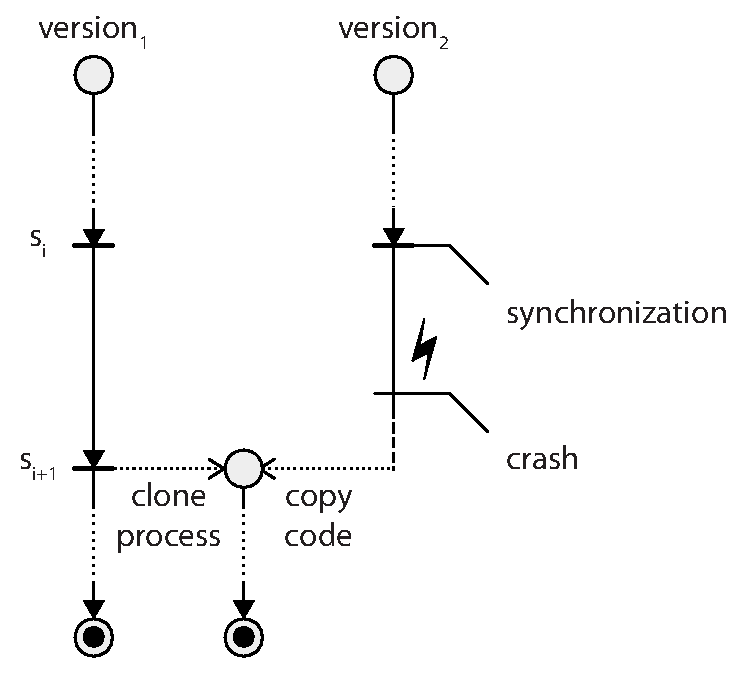
\includegraphics[width=0.45\columnwidth]{safe-updates/figures/solution1}
%%     \label{fig:solution1}
%%   }
%%   \quad
%%   \subfloat[Patch state before the crash and continue execution]{
%%     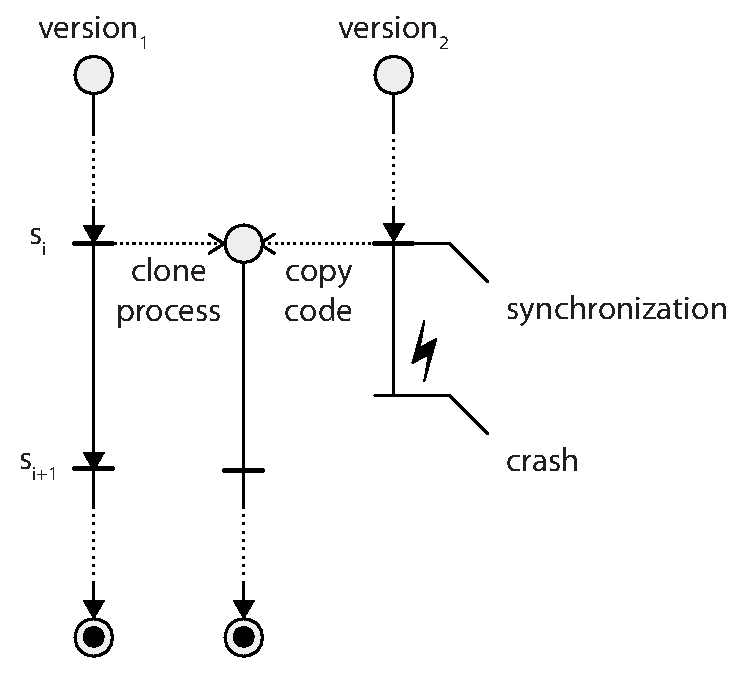
\includegraphics[width=0.45\columnwidth]{safe-updates/figures/solution2}
%%     \label{fig:solution2}
%%   }
%%   \\
%%   \subfloat[Use the code of older version only to run through critical section]{
%%     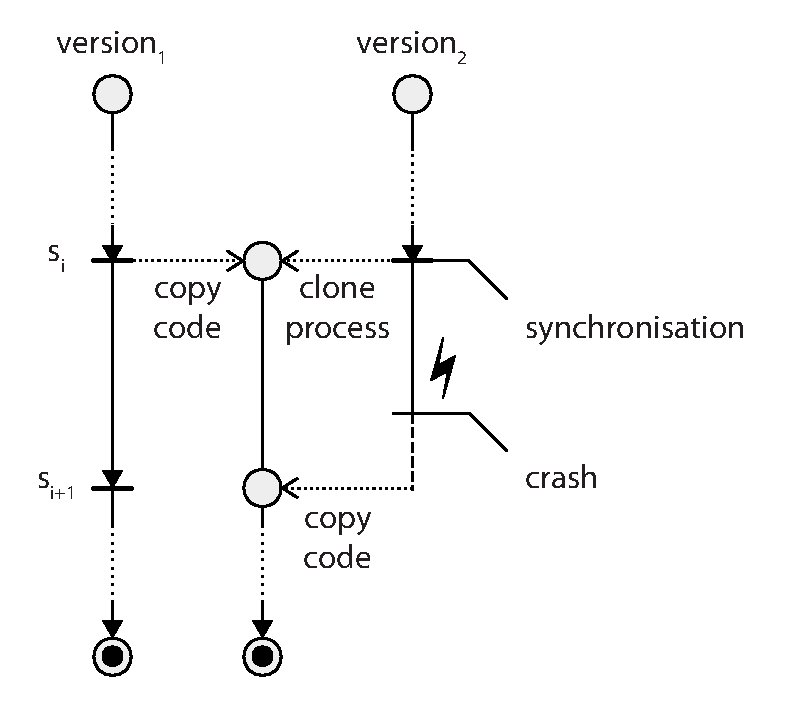
\includegraphics[width=0.45\columnwidth]{safe-updates/figures/solution3}
%%     \label{fig:solution3}
%%   }
%%   \caption{Three solutions for synchronising two divergent versions of
%%   the same application}
%%   \label{fig:solution}
%% \end{figure}

%% \item\label{s1} Clone the correctly executing version to duplicate its state
%%   (\eg memory content, memory mappings) after the crash and replace its
%%   code with the code of the failed version. Then restart both versions and
%%   continue their execution (Figure~\ref{fig:solution1}).

%% \item\label{s2} Clone the correctly executing version to duplicate its state
%%   (\eg memory content, memory mappings) at the last synchronisation point (\ie
%%   creating checkpoint). After the crash, replace the code of this cloned
%%   version with the code of the failed version. Then restart this cloned
%%   version, execute over the \emph{critical section}, and continue execution of
%%   both versions (Figure~\ref{fig:solution2}).

%% \item\label{s3} Clone the failing version to duplicate its state (\eg memory
%%   content, memory mappings) at the last synchronisation point (\ie creating
%%   checkpoint). After the crash, replace the code of this cloned version with
%%   the code of the correctly executing version. Then restart this cloned
%%   version; after the application successfully executes over the \emph{critical
%%   section}, replace the code of the cloned version again with the original
%%   code, and continue its execution (Figure~\ref{fig:solution3}).

%% \end{enumerate}

Our exact recovery mechanism is illustrated in
Figure~\ref{fig:solution3}.  At each system call, \mx creates a
lightweight checkpoint of each version.  This is implemented using the
\textstt{clone} system call in Linux, which internally uses a
copy-on-write strategy.  
%% As an important optimisation, we omit system
%% calls that can be replayed safely from the last checkpoint, such
%% as \textstt{read}.

As shown in Figure~\ref{fig:solution3}, suppose that the crash happens
in version $v_2$, between system calls $s_1$ and $s_2$.  Then, \rem
first restores $v_2$ at point $s_1$, copies $v_1$'s code into $v_2$'s
code segment, executes over the buggy code using $v_1$'s code (but
note that we are still using $v_2$'s memory state), and then restore
$v_2$'s code at point $s_2$.

There are several challenges in implementing this functionality.
First, \rem needs the ability to read and write the application code
segment.  In the current implementation, we bypass this by linking
together the two application versions after renaming all the symbols
in one of the versions using a modified version of
the \textstt{objcopy}
tool.\footnote{\url{http://sourceware.org/binutils/docs/binutils/objcopy.html}}
However, in the future we plan to implement this transparently by
using the cross-memory attach mechanism used by \mxm.
%% \textstt{pread} and \textstt{pwrite} interface to directly
%% read and write the process memory via the
%% %\textstt{/proc/<pid>/mem} file in the
%% \emph{proc} file system.

%% This functionality has been recently introduced to the Linux kernel in
%% version 2.6.39~\cite{kernel-procmem}; previously, this interface was
%% read-only. This approach imposes only minimal overhead as it allows
%% direct access to the process memory space.

%% The runtime process manipulation functionality is implemented inside
%% \rem, a separate component used by the \mxm monitor. The
%% manipulation itself is driven by the data obtained statically by the
%% \sea analyser before the application has been executed.

Second, \rem needs to modify the contents of the stack in $v_2$.  This
is necessary because the return addresses on the stack frames of $v_2$
still point to $v_2$'s original code, which was now replaced by
$v_1$'s code.  Without also modifying $v_2$'s stack, any
function \textstt{return} instruction executed between $s_1$ and $s_2$
would most likely veer execution to an incorrect location, since
function addresses are likely to be different across different
versions.  Thus, after \rem replaces $v_2$'s code, it also updates the
return addresses on $v_2$'s stack with the corresponding return
addresses in $v_1$, which are obtained via static analysis
(\S\ref{sec:sea}).  Because system calls are invoked via wrapper
functions in \textstt{libc}, this ensures that when $v_2$ resumes
execution, it will immediately return to the code in $v_1$.
%% \rem obtains these addresses by analysing $v_1$'s stack at
%% position $s_1$ accessible via checkpoint taken at that point.
%
To implement this functionality, \rem makes use of
the \textstt{libunwind}
library,\footnote{\url{http://www.nongnu.org/libunwind/}} which provides a
portable interface for accessing the program stack, for both x86 and
x86-64 architectures. To actually modify the execution stack of
$v_2$, \rem uses again the \ptrace interface.


Unfortunately, updating the stack return addresses is not sufficient
to ensure that $v_2$ uses $v_1$'s code between $s_1$ and $s_2$, as
$v_2$ may also use function pointers to make function calls.
%% Note that we are still using the $v_2$ memory state. Thereby, $v_2$
%% may still issue a function call to the original code through one of
%% the function pointers.
To handle such cases, \rem inserts breakpoints to the first
instruction of every function in $v_2$'s original code.  Then, when a
breakpoint is encountered, \rem is notified via a \textstt{SIGTRAP}
signal, and redirects execution to the equivalent function in $v_1$'s
code (which is obtained from the \sea component) by simply changing
the instruction pointer.
%The address of the equivalent function is obtained

Finally, after executing through the buggy code, \rem performs the
same operations in reverse: it redirects execution to $v_2$'s original
code, changes the return addresses on the stack to point to $v_2$'s
functions, and disables all breakpoints inserted in $v_2$'s code.  
The one additional operation that is done at this point is to copy all
the global data modified by $v_1$'s code into the corresponding
locations referenced by $v_2$'s code.  

%\paragraph{Runtime stack analysis and manipulation.}

%% For example, on the x86 architecture, the stack can be easily
%% traversed starting from the top as each stack frame contains frame
%% pointer pointing to the previous stack frame, thereby forming a linked
%% list-like structure. This is not possible on the x86-64 architecture
%% as the frame pointer is no longer stored inside the stack frame.  To
%% traverse the execution stack on this architecture, it is necessary to
%% compute sizes of all functions' stack frames using the stack usage
%% information stored in the \texttt{UNWIND\_CODE} section, which is a
%% part of the ELF binary file. This logic is implemented by the
%% \texttt{libunwind} library, which provides API to unwind the stack
%% independent of the target platform.

%The necessary information about the stack location (\ie address range) and
%page mapping are obtained through the \emph{proc} file system; in particular
%the \textstt{/proc/<pid>/maps} and \textstt{/proc/<pid>/pagemap} files.

Note that \mx cannot currently handle major modifications to the
layout of the data structures used by the code, including individual
stack frames.  While this still allows us to support several common
software update scenarios, in future work we plan to improve the
system with the ability to perform full stack
reconstruction~\cite{upstare} and automatically infer basic data
structure changes at the binary-level~\cite{data-struct-digging}.
%% to identify changes to function names and sequences of function calls
%% (e.g., via clone detection techniques~\cite{cp-miner06,deckard07}),


Our approach of using the code of the non-crashing version to survive
failures in the crashing one may potentially leave the recovered
version in an inconsistent state. However, \mx is able to discover
most internal state inconsistencies by comparing whether the two
versions have the same external behaviour. When the behaviour of the
recovered version starts to differ, \mx will immediately discard it
and continue with only one version. The discarded version can be later
restarted at a convenient synchronisation point.  This restarting
functionality is not currently implemented in \mx, but we plan to add it
as a future extension.

%Our approach of using the code of the non-crashing version to survive
%failures in the crashing one may leave the application in an
%inconsistent state, and thus may not be applicable for application in
%which absolute correctness and a fail-fast approach are more important
%than allowing the application to survive errors.  However, \mx is
%usually able to discover most internal state inconsistencies, since it
%regularly checks if the two versions have the same external
%behaviour. (See \S\ref{sec:discussion} for an extended discussion.)

\subsection{Binary static analysis}
\label{sec:sea}

%% \begin{table*}[t]
%% \centering 
%% \begin{tabular}{ccc}
%%   \hline
%%   Library calls in $\mathrm{version}_1$ & Library calls in $\mathrm{version}_2$ &
%%   System calls within the library \\
%%   \hline
%%   \texttt{<0xdeadbe5a>} & \texttt{<0xdeadbe8e>} &
%%   [\texttt{<0x77ff2c>}, \texttt{<0x77ffae>}] \\
%%   \texttt{<0xdeadabf5>} & \texttt{<0xdeadac34>} &
%%   [\texttt{<0x782bae>}] \\
%%   \vdots & \vdots & \vdots \\
%% \end{tabular}
%% \caption{Addresses of library function calls, and system calls invoked from
%% within these functions.}
%% \label{tab:syscall_table}
%% \end{table*}

The \sea component statically analyses the binaries of the two
versions to obtain information needed at runtime by the \mxm and \rem
components.  \sea is invoked only once, when the multi-version
application is assembled from its component versions.
%% As mentioned in \sref{sec:rem}, we currently link together the
%% two application versions after renaming all the symbols in one of them
%% using a modified copy of the \textstt{objcopy} tool, although in the
%% future we plan to do this linking dynamically by directly changing the
%% code segment in each version.

The main goal of \sea is to create several mappings from the code of
one version to the code of the other.  First, \sea extracts the
addresses of all function symbols
in one version and maps them to the
addresses of the corresponding functions in the other version.  This
mapping is used by \rem to handle calls performed via function
pointers (\S\ref{sec:rem}).

Second, \sea computes a mapping from all possible return addresses in
one version to the corresponding return addresses in the other version.  In
order to allow for code changes, this mapping is done by computing an
ordered list of all possible return addresses in each function.  For
example, if function \textstt{foo} in $v_1$ performs call instructions
at addresses \textstt{0xabcd0000} and \textstt{0xabcd0100}, and
function \textstt{foo} in $v_2$ performs call instructions at
addresses \textstt{0xdcba0000} and \textstt{0xdcba0400}, then \sea
will compute the mapping \textstt{\{0xabcd0005 $\rightarrow$
0xdcba0005, 0xabcd0105 $\rightarrow$ 0xdcba0405\}} (assuming each call
instruction takes 5 bytes).  This mapping is then used by \rem to
rewrite return addresses on the stack.

%% These data are gathered by the \sea analyser component which
%% implements static analysis of binary executables to extract all
%% necessary addresses and provide them to other components inside our
%% system. The format used for storing these data is represented by a
%% \emph{call table}. For each version, this table contains addresses of
%% all calls to shared library functions together with the list of all
%% system calls addresses invoked within these library functions, as can
%% be seen in Table~\ref{tab:syscall_table}.

%% For example, the first line of this table represents a call to a
%% library function which does two system calls, while second line
%% represents a function call which does only one system call.

To construct these tables, \sea first needs to extract the addresses
of all function symbols and then disassemble the code for each
individual function in order to locate the call instructions within
them.  The implementation is based on the \textstt{libbfd}
and \textstt{libopcodes} libraries, which are 
part of the
\gnu \binutils suite.\footnote{\url{http://www.gnu.org/software/binutils/}}
To obtain the addresses of all function symbols defined by the
program, \sea uses \textstt{libbfd} to extract the static and dynamic
symbol tables and relocation tables.  To disassemble individual
functions, \sea uses the \textstt{libbf}
library,\footnote{\url{http://github.com/petrh/libbf}} 
built on top of \textstt{libopcodes}.

%% Disassembled machine code is stored in a graph-like structure where
%% individual instructions represents vertices and edges between these
%% vertices represents the control flow. 

%% \paragraph{System call identification.}
%% \sea implementation uses the disassembler to obtain machine
%% code of each individual function and iterates over its instructions
%% (traversing the instruction graph) to identify basic blocks and locate
%% system call instructions within the code these functions.

%% To locate system calls within shared library function calls,
%% \sea first needs to obtain the set of exported library
%% functions and system calls within these functions using the above
%% described approach. Then, \sea analyses the application binary
%% itself and locates all function calls to the shared library using the
%% information extracted from relocation and procedure lookup tables
%% contained in ELF binaries.

%% Results of this analysis are stored in a hash table and tree structure
%% to allow quick access eliminating any unnecessary overhead when these
%% information are accessed during runtime. These data are then used to
%% construct the already described \emph{call table}, before the
%% application itself is executed.

%% \subsection{Limitations and Future Work}
%% \label{sec:limitations}
%% \input{limitations}
